%-------------------------------------------------------------------------------
% yum_addsynth
%-------------------------------------------------------------------------------
%
% \file        yum_addsynth.tex
% \library     Documents
% \author      Chris Ahlstrom
% \date        2015-06-07
% \update      2019-12-21
% \version     $Revision$
% \license     $XPC_GPL_LICENSE$
%
%     Provides the ADDsynth section of yoshimi-user-manual.tex.
%
%-------------------------------------------------------------------------------

\section{ADDsynth}
\label{sec:addsynth}

   The \textsl{Yoshimi} ADDsynth (also spelled "ADsynth" or "AddSynth")
   dialog is a complex dialog for creating an
   instrument.  This is the most complex, most advanced and most
   sophisticated part of the synthesizer and allows one to edit the
   parameters that apply to all the voices of ADDsynth.

   ADDsynth, a primarily additive synthesis engine, is one of the three major
   synthesis engines available in \textsl{Yoshimi}/\textsl{ZynAddSubFX}.
   The basic concept of this engine is the summation of a collection of voices,
   each of which consists of oscillators.

   "ADDsynth" (sometimes spelled "ADsynth") or "ADnote" is a complex engine
   which makes sounds by adding a number of voices. Each one has filters,
   envelopes, LFOs, morphing, modulation, resonance, etc.
   Each voice includes a very powerful
   waveform generator with up to 128 sine/non-sine harmonics. One can use
   Fourier synthesis, or if one doesn't like it, one can use
   wave-shaping/filtering of functions. This engine includes anti-aliasing.
   Modulation includes ring modulation, phase modulation, and more.
   The modulators can have any shape.
   \cite{zyndoc}

   There are two oscillators per voice: the \index{voice oscillator} voice
   oscillator and the \index{modulation oscillator} modulation oscillator. For
   each of these two oscillators, there are three alternatives: one can have a
   locally defined oscillator (internal), an oscillator defined in a
   lower-numbered voice or use a lower-numbered voice itself as an oscillator
   (that voice must be enabled).

   In the voice window, each of the two oscillators has a \textbf{Source} and a
   \textbf{Local Oscillator}. The \textbf{Source} gives the choice of previous
   voices as oscillators and the \textbf{Local Oscillator} gives the choice
   of previously defined oscillators and the current (internal) oscillator.

   The sum of the voices are passed through filters and amplification to
   produce the final sound. This could lead one to think that ADDsynth is just
   a bunch of minor post-processing, and at this level much of the sound
   generation is hidden.

\begin{figure}[H]
   \centering
   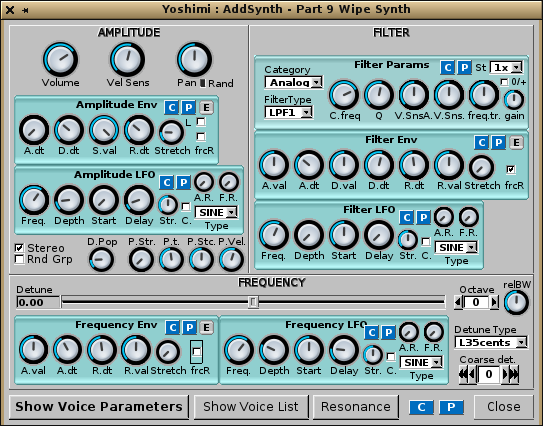
\includegraphics[scale=1.0]{2.0/AddSynth.png}
   \caption{ADDsynth Edit/Global Dialog}
   \label{fig:addsynth_edit_dialog}
\end{figure}

   The major sections of this dialog are listed:

   \begin{enumber}
      \item \textbf{AMPLITUDE} (stock section)
      \item \textbf{FILTER} (stock section)
      \item \textbf{FREQUENCY} (stock section)
      \item \textbf{Show Voice Parameters} (section)
      \item \textbf{Show Voice List} (section)
      \item \textbf{Resonance} (stock section)
      \item \textbf{C}
      \item \textbf{P}
      \item \textbf{Close}
   \end{enumber}

   This complex dialog is best described section by section.
   Many of the sub-sections are stock sub-panels described elsewhere
   in this document.  References to those sections are included.

\subsection{ADDsynth / AMPLITUDE}
\label{subsec:addsynth_amplitude}

   \begin{enumber}
      \item \textbf{Volume}
      \item \textbf{Vel Sens}
      \item \textbf{Pan}
      \item \textbf{Rand}
      \item \textbf{Width}

       The controls above are discussed in detail in
       \sectionref{subsec:volume_panning}. However their values for ADDsynth
       are as below.

      \item \textbf{Amplitude Env}
         The Amplitude Env panel is described in detail in
         \sectionref{subsubsec:amplitude_envelope_subpanel}.
      \item \textbf{Amplitude LFO}
         The Amplitude LFO panel is described in detail in
         \sectionref{subsubsec:lfo_user_interface_panels}.

      \item \textbf{Stereo}
      \item \textbf{Rnd Grp}
      \item \textbf{P.Str.}
      \item \textbf{P.t}
      \item \textbf{P.Stc.}
      \item \textbf{P.Vel.}
   \end{enumber}

   Note the two sub-panels, mentioned above, that are described elsewhere.
   They will not be discussed in detail below.

   \setcounter{ItemCounter}{0}      % Reset the ItemCounter for this list.

   \itempar{Volume}{addsynth!volume}

   Values: \texttt{-60dB to 19.4dB, -3.8dB*}

   \itempar{Vel Sens}{addsynth!vel sens}

   Values: \texttt{-48dB to -0.8dB, disabled, -6.02dB*}

   \itempar{Pan}{addsynth!pan}

   Values: \texttt{100\% left to 100\% right, centered*}

   \itempar{Rand}{addsynth!random pan}

   Values: \texttt{off*, on}

   \itempar{Width}{addsynth!random width}

   Values: \texttt{0 to 100\%* }

   Next, we skip the \textbf{Amplitude Env} and \textbf{Amplitude LFO}
   panels, which are described elsewhere, as noted above.

   \itempar{Stereo}{addsynth!Stereo}
   ADDsynth Stereo.
   Stereo can be enabled.
   When disabled, all the voices will also have panning disabled.

   Values: \texttt{Off, On*}

   \itempar{Rnd Grp}{addsynth!group}
   ADDsynth Random Group.
   Disable harmonic amplitude randomness of voices with a common oscillator.
   There are many per-voice random elements that can give the sound more
   'depth'. When this control is checked, the voices all sound together
   instead.

   Values: \texttt{Off*, On}

   \itempar{P.Str}{addsynth!punch strength}
   ADDsynth Punch Strength.
   The punch strength of a note in ADDsynth is a constant amplification to
   the output at the start of the note, with its length determined by the
   punch time and stretch and the amplitude being determined by the punch
   strength and velocity sensing. The \textbf{relBW}
   control in the frequency panel is
   effectively a multiplier for detuning all voices within an ADnote.

   Values: \texttt{0* to 127}

   \itempar{P.t}{addsynth!punch time}
   ADDsynth Punch Time (duration).
   Sets the punch effect duration (from 0.1 ms to 100 ms on an A note, 440Hz).

   Values: \texttt{0 to 127, 64*}

   \itempar{P.Stc}{addsynth!punch stretch}
   ADDsynth Punch Stretch.
   Sets the punch effect stretch according to frequency. On lower-frequency
   notes, punch stretch makes the punch effect last longer.

   Values: \texttt{0 to 127, 64*}

   \itempar{P.Vel}{addsynth!punch vel sens}
   ADDsynth Punch Velocity Sensing.
   The higher this value, the higher the effect of velocity on the punch of
   the note.

   Values: \texttt{0 to 127, 72*}

\subsection{ADDsynth / FILTER}
\label{subsec:addsynth_filter}

   The ADDsynth FILTER block consists solely of sub-panels
   described in detail in the sections noted below.  The
   sub-panels of the FILTER section are:

   \begin{enumber}
      \item \textbf{Filter Params}
      \item \textbf{Filter Env}
      \item \textbf{Filter LFO}
   \end{enumber}

   \setcounter{ItemCounter}{0}      % Reset the ItemCounter for this list.

   \itempar{Filter Params}{addsynth!filter params}
   ADDsynth Filter Parameters.
   The Filter Params panel is described in detail in
   \sectionref{subsubsec:filter_parameters_user_interface}.

   \itempar{Filter Env}{addsynth!filter env}
   ADDsynth Filter Envelope.
   The Filter Env panel is described in detail in
   \sectionref{subsubsec:envelope_settings_for_filter}.

   \itempar{Filter LFO}{addsynth!filter lfo}
   The Filter LFO panel is described in detail in
   \sectionref{subsubsec:lfo_user_interface_panels}.

\subsection{ADDsynth / FREQUENCY}
\label{subsec:addsynth_frequency}

   \begin{enumber}
      \item \textbf{Detune}
      \item \textbf{FREQUENCY slider}
      \item \textbf{Octave}
      \item \textbf{RelBW}
      \item \textbf{Frequency Env}.
         A stock sub-panel described in
         \sectionref{subsubsec:envelope_settings_for_frequency}.
      \item \textbf{Frequency LFO}
         A stock sub-panel described in
         \sectionref{subsubsec:frequency_lfo_sub_panel}.
      \item \textbf{Detune Type}
      \item \textbf{Coarse det.}
   \end{enumber}

   \setcounter{ItemCounter}{0}      % Reset the ItemCounter for this list.

   \itempar{Detune}{addsynth!detune value}
   ADDsynth Detune Value.
   This display box shows the value of the detune as selected by the
   frequency slider described below.

\begin{figure}[H]
   \centering
   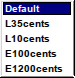
\includegraphics[scale=1.0]{bottom-panel/instrument-edit/ADD/frequency-detune-type.jpg}
   \caption{ADDsynth Frequency Detune Type}
   \label{fig:addsynth_freq_detune_type}
\end{figure}

   This value defines the number of cents that define the range of the
   \textbf{FREQUENCY} slider, that is 35 cents, 10 cents, 100 cents (one
   semitone), or 1200 cents (1 octave), below and above the main
   frequency.  The default is 35 cents.  The 1200-cents setting provides a
   whole octave of detuning in either direction.

   The "L" stands for "linear", and the "E" for "exponential", to
   describe how the detune slider acts.

   Values: \texttt{Default*, L35cents, L10cents, E100cents, E1200cents}

   \itempar{FREQUENCY slider}{addsynth!freq slider}
   ADDsynth Fine Detune (cents), a slider control.
   While the detune type dropdown and the octave selection provide a coarse
   selection of detune, the slider allows for a finer selection of detune,
   up to roughly one-third of a semitone.

   Values:
      \texttt{-35.00 to 35.00},
      \texttt{-10.00 to 10.00},
      \texttt{-100.00 to 100.00},
      \texttt{-1200.00 to 1200.00}

   \itempar{Octave}{addsynth!octave}
   ADDSynth Octave.
   The octave setting changes the frequency by octaves.

   Values: \texttt{-8 to 7, 0*}

   \itempar{RelBW}{addsynth!relative bw}
   ADDSynth Relative Bandwidth.
   Bandwidth: how the relative fine detune of the voice is changed.

   Values: \texttt{0 to 127, 64*}

   \itempar{Frequency Env}{addsynth!frequency env}
   ADDsynth Frequency Envelope.
   The Frequency Env panel is described in detail in
   \sectionref{subsubsec:envelope_settings_for_frequency}.

   \itempar{Frequency LFO}{addsynth!frequency lfo}
   The Frequency LFO panel is described in detail in
   \sectionref{subsubsec:lfo_user_interface_panels}

   \itempar{Detune Type}{addsynth!detune type}
   Frequency Detune Type.
   This setting provides a coarse detuning.
   We would welcome an explanation of exactly is meant by the numbers and
   the "E" versus "L" designation.

   Values: \texttt{L35cents, L10cents, E100cents, E1200cents}

   \itempar{Coarse det}{addsynth!coarse detune}
   Coarse Detune, "C.detune".
   The one-arrow buttons change the value by one.
   The two-arrow buttons change the value by ten.
   Again, we need a way to explain the interactions of the slider, the
   octave setting, the detune type, and the coarse detune settings.

   Values: \texttt{-64 to 63, 0*}

   \itempar{Show Voice Parameters}{addsynth!voice parameters}
   ADDsynth Show Voice Parameters.
   This button brings up the "voice parameters" dialog discussed in the next
   section.

\subsection{ADDsynth / Voice Parameters}
\label{subsec:addsynth_voice_parameters}

   Again, this dialog is built from some stock sections and stock
   sub-panels, plus additional elements.

   Each \textsl{Yoshimi} ADDsynth instrument consists of up to 8 voices.
   This dialog provides a way to define each of the 8 voices in great
   detail.  By default, an ADDsynth instrument consists of one voice, voice 1.

\begin{figure}[H]
   \centering
   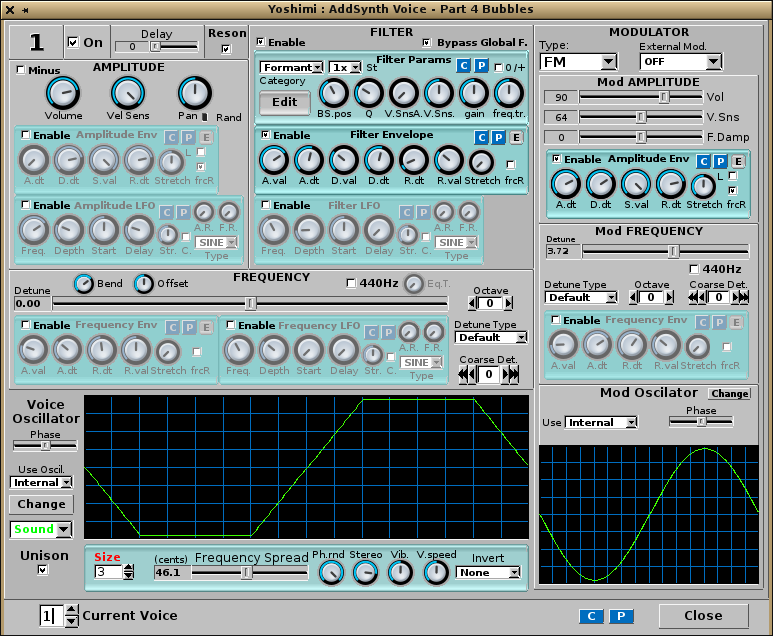
\includegraphics[scale=0.75]{2.0/AddVoice.png}
   \caption{ADDsynth Voice Parameters Dialog}
   \label{fig:addsynth_voice_parameters_dialog}
\end{figure}

   Note the 8 \textbf{VOICE} tabs at the top of the window.
   These make it easy to switch to another voice, and without opening up yet
   another editing window.
   Non-active voices are shown with an inactive tab/number appearance.
   This is all in synchrony with the \textbf{Voice List} window.

   This dialog consists of a few extra settings, plus a number of
   stock dialog sections.  Take some time to compare
   \figureref{fig:addsynth_edit_dialog},
   which covers the overall instrument, with
   \figureref{fig:addsynth_voice_parameters_dialog},
   which covers each of the voices.
   The stock sections in the former cover the whole instrument as one,
   while the very similar stock sections in the latter cover only the
   voice they configure.
   Obviously, the combinations of settings are essentially endless.

   Each voice can be amplitude-controlled, filter-controlled, and
   frequency-controlled.  Each voice can also be modulated by a
   modulator.

  Another property of the voice is that one can tell \textsl{Yoshimi} to
  import a given lower-numbered voice, either as an oscillator, or as a
  modulator.

   \begin{enumber}
      \item \textbf{Voice Number Tab}
      \item \textbf{On}
      \item \textbf{Delay}
      \item \textbf{Resonance}
      \item \textbf{AMPLITUDE} (see the stock-panel section below)
      \item \textbf{FILTER} (see the stock-panel section below)
      \item \textbf{MODULATOR} (see the stock-panel section below)
      \item \textbf{FREQUENCY} (see the stock-panel section below)
   \end{enumber}

   \setcounter{ItemCounter}{0}      % Reset the ItemCounter for this list.

   \itempar{Voice Number Tab}{voice!number}
   ADDsynth Voice Number.
   When highlighted this indicates the voice currently being viewed.  Each
   \textsl{Yoshimi} part/instrument can consist of up to eight voices. The
   voice being worked on can be selected using the \textbf{Current Voice} tab.

   Values: \texttt{1* to 8}

   \itempar{On}{voice!on/off}
   ADDsynth Voice On/Off.
   Enables this voice in the part/instrument.

   Values: \texttt{Off, On}

   \itempar{Delay}{voice!delay}
   ADDsynth Voice Delay.
   \index{todo!voice delay units (milliseconds/seconds)}

   Values: \texttt{0* to 4.90 s}

   \itempar{Resonance}{voice!resonance}
   ADDsynth Voice Resonance On/Off.
   The rest of the GUI elements
   (AMPLITUDE, FILTER, MODULATOR, FREQUENCY, and Voice Oscillator)
   are more detailed, and discussed in the sections that follow.

   Values: \texttt{Off, On*}

\subsubsection{ADDsynth / Voice Parameters / AMPLITUDE}
\label{subsubsec:addsynth_voice_parameters_amplitude}

   This section of the voice parameters dialog also includes a couple of
   stock sub-panels that have an additional "Enable" control.

   \begin{enumber}
      \item \textbf{Minus}
      \item \textbf{Volume}
      \item \textbf{Vel Sens}
      \item \textbf{Pan}
      \item \textbf{Rand}
      \item \textbf{Width}

      The controls above are discussed in detail in
       \sectionref{subsec:volume_panning}. However their values for ADDsynth
       Voice are as below.

      \item \textbf{Amplitude Env, Stock + Enable}
      \item \textbf{Amplitude LFO, Stock + Enable}
   \end{enumber}

   \setcounter{ItemCounter}{0}      % Reset the ItemCounter for this list.

   \itempar{Minus}{voice par amp!invert phase}
   ADDsynth Amplitude Minus.
   When checked, this control inverts the phase of the waveform relative to
   all the other voices.
   With only one voice enabled, this control will seem to do nothing.
   With two voices enabled with \textsl{identical} waveforms, the
   \textbf{Minus} control will indeed seem to reverse the effect of the volume
   control. But if the waveforms are different, then it can provide some
   interesting harmonic change effects.

   Values: \texttt{Off*, On}

   \itempar{Volume}{voice par amp!volume}

   Values: \texttt{off, -57.6dB to 0dB, -12.8dB*}

   \itempar{Vel Sens}{voice par amp!vel sens}

   Values: \texttt{-48dB to -0.8dB, disabled*}

   \itempar{Pan}{voice par amp!pan}

   Values: \texttt{100\% left to 100\% right, centered*}

   \itempar{Rand}{voice par amp!random pan}

   Values: \texttt{off*, on}

   \itempar{Width}{voice par amp!random width}

   Values: \texttt{0 to 100\%* }

   \itempar{Amplitude Env, Stock + Enable}{voice par amp!amp env}
   ADDsynth Amplitude Envelope Sub-panel.
   See \sectionref{subsubsec:amplitude_envelope_subpanel}.
   Additionally, the \textbf{Enable} checkbox allows the enabling of this
   component.

   \itempar{Amplitude LFO, Stock + Enable}{voice par amp!amp lfo}
   ADDsynth Amplitude LFO Sub-panel.
   See \sectionref{subsubsec:lfo_user_interface_panels}.
   Additionally, the \textbf{Enable} checkbox allows the enabling of this
   component.

\subsubsection{ADDsynth / Voice Parameters / FILTER}
\label{subsubsec:addsynth_voice_parameters_filter}

   This section of the voice parameters dialog also includes a couple of
   stock sub-panels that have an additional "Enable" control.

   \begin{enumber}
      \item \textbf{Enable}
      \item \textbf{Bypass Global F.}
      \item \textbf{Filter Params, Stock}
      \item \textbf{Filter Env, Stock + Enable}
      \item \textbf{Filter LFO, Stock + Enable}
   \end{enumber}

   \setcounter{ItemCounter}{0}      % Reset the ItemCounter for this list.

   \itempar{Enable}{voice par filter!enable}
   ADDsynth Voice Enable Filter.
   This value enables the whole FILTER dialog section.

   Values: \texttt{Off*, On}

   \itempar{Bypass Global F}{voice par filter!bypass}
   ADDsynth Voice Bypass Global Filter.
   The voice signal bypasses the global filter.

   Values: \texttt{Off*, On}

   \index{todo!global filter}
   We need to make sure there is a discussion of the global filter.

   \itempar{Filter Params, Stock}{voice par filter!parameters}
   See \sectionref{subsubsec:filter_parameters_user_interface}.

   \itempar{Filter Env, Stock + Enable}{voice par filter!env}
   See \sectionref{subsubsec:envelope_settings_for_filter}.

   \itempar{Filter LFO, Stock + Enable}{voice par filter!lfo}
   See \sectionref{subsubsec:filter_lfo_sub_panel}.

\subsubsection{ADDsynth / Voice Parameters / FREQUENCY}
\label{subsubsec:addsynth_voice_parameters_frequency}

   This frequency section is almost a stock part.
   It is similar to the ADDsynth Edit's \textbf{FREQUENCY} section.

   \begin{enumber}
      \item \textbf{Detune}
      \item \textbf{FREQUENCY slider}
      \item \textbf{440Hz}          % addition to stock
      \item \textbf{Eq.T}          % addition to stock
      \item \textbf{Octave}
      \item \textbf{Detune Type}
      \item \textbf{Coarse det}
      \item \textbf{Frequency Env, Stock + Enable}
      \item \textbf{Frequency LFO, Stock + Enable}
      \item \textbf{Voice Oscillator}
   \end{enumber}

   \setcounter{ItemCounter}{0}      % Reset the ItemCounter for this list.

   \itempar{Detune}{voice parameters!detune}
   Voice Parameters Detune.
   Shows the value selected by the frequency slider.

   \itempar{FREQUENCY slider}{voice parameters!freq slider}
   Frequency Slider.
   Provides fine detune, in cents.
   Note that 35 cents is roughly one-third of a semitone.

   Values: \texttt{-35.00 to 35.00, 0*}

   \itempar{440Hz}{voice parameters!440 hz}
   440 Hz Selection.
   Fixes the voice base frequency to 440 Hz.
   One can adjust this with the detune settings.
   No matter what key is played on the keyboard, this voice will emit only
   440 Hz.  This is useful for defining a constant frequency to use as a
   modulator for the other voices in the part.
   For example, one can define voice 1 to be a tone, then
   define voice 2 to be 440 Hz.  The two voices will mix, but only voice 1
   will change frequencies as different keys are played.

   Values: \texttt{Off*, On}

   \itempar{Eq.T}{voice parameters!eq type}
   Equal Temperament
   This item is enabled only if the \textbf{440Hz} check-box is enabled.
   If this is greater than zero it modifies the effect of the 440Hz checkbox. The A4
   key remains at 440Hz, but the frequency of the other keys vary according to the
   key pressed. When set to the middle of the value range (64), the step size is
   exactly like the classical equal temperament, i.e. one note step for one semitone
   and 12 steps will double the frequency.

   Values: \texttt{0 to 127}

   \itempar{Octave}{voice parameters!octave}
   Voice Parameters Octave.

   Values: \texttt{-8 to 7, 0*}

% Where did I get this setting?  An older version of the dialog?
%
%  \itempar{RelBW}{voice parameters!relbw}
%  Relative bandwidth.

   \itempar{Detune Type}{voice parameters!fine detune}
   Detune Type.

\begin{figure}[H]
   \centering
   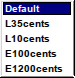
\includegraphics[scale=1.0]{bottom-panel/instrument-edit/ADD/frequency-detune-type.jpg}
   \caption{Frequency Detune Type}
   \label{fig:frequency_detune_tYpe}
\end{figure}

   Values: \texttt{Default*, L35cents, L10cents, E100cents, E1200cents}

   \itempar{Coarse det}{voice parameters!coarse detune}
   Coarse Detune.
   Is this setting in units of semitones?
   \index{todo!coarse detune units}

   Values: \texttt{-64 to 63, 0*}

   \itempar{Frequency Env, Stock + Enable}{voice parameters!freq env}
   Frequency Envelope.
   See \sectionref{subsubsec:envelope_settings_for_frequency}.

   \itempar{Frequency LFO, Stock + Enable}{voice parameters!freq lfo}
   Frequency LFO.
   See \sectionref{subsubsec:frequency_lfo_sub_panel}.

   \itempar{Voice Oscillator}{voice parameters!oscillator}
   Voice Parameters Oscillator.
   See the next section.

\subsubsection{ADDsynth / Voice Parameters / UNISON}
\label{subsubsec:addsynth_voice_parameters_unison}
   Enabling this item causes the Unison-related items to become
   activated.

   \begin{enumber}
      \item \textbf{On}
      \item \textbf{Size}
      \item \textbf{Frequency Spread}
      \item \textbf{Ph.rnd}
      \item \textbf{Stereo}
      \item \textbf{Vib.}
      \item \textbf{V.speed}
      \item \textbf{Invert}
   \end{enumber}

   \setcounter{ItemCounter}{0}      % Reset the ItemCounter for this list.

   \itempar{On}{unison!enable}
   Enables or disables unison. When disabled the size is always set at 2.

   Values: \texttt{Off*, On}

   \itempar{Unison Size}{unison!size}
   Sets the number of unison sub-voices.

   Values: \texttt{2* to 50}

   \itempar{Unison Frequency Spread}{unison!freq spread}
   Frequency spread of the unison (cents).

   Values: \texttt{0 to 200, 44.6*}

   \itempar{Phase Randomness}{unison!Ph.rnd}
   Unison Phase Randomness.

   Values: \texttt{0 to 127*}

   \itempar{Stereo Spread}{unison!Stereo}
   Unison Stereo Spread.

   Values: \texttt{0 to 127, 64*}

   \itempar{Unison Vibrato}{unison!Vibrato}
   Unison Vibrato.

   Values: \texttt{0 to 127, 64*}

   \itempar{Vibrato Speed}{unison!V.speed}
   Unison Vibrato Average Speed.

   Values: \texttt{0 to 127, 64*}

   \itempar{Phase Invert}{unison!Invert}
   Unison Phase Invert.
   Values: \texttt{None*, Random, 50\%, 33\%, 25\%, 20\%}

\begin{figure}[H]
   \centering
   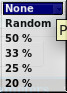
\includegraphics[scale=1.0]{bottom-panel/instrument-edit/ADD/voice-oscillator-phase-invert-dropdown.jpg}
   \caption{Unison Phase Invert Dropdown}
   \label{fig:phase_invert_dropdown}
\end{figure}


\subsubsection{ADDsynth / Voice Parameters / Voice Oscillator}
\label{subsubsec:addsynth_voice_parameters_oscillator}

   The ADDsynth Voice Oscillator panel is tucked in the lower left side of the
   ADDSynth Voice Parameters editor.

   \begin{enumber}
     \item \textbf{Voice}
      \item \textbf{Sound}
      \item \textbf{Waveform graph}
      \item \textbf{Use}
      \item \textbf{Waveform} (was Change)
      \item \textbf{Phase}
      \item \textbf{C}
      \item \textbf{P}
      \item \textbf{Close Window}
   \end{enumber}


   \setcounter{ItemCounter}{0}      % Reset the ItemCounter for this list.

  \itempar{Source}{voice oscillator!Source}
  ADDSynth Voice Import. Selects whether to import a lower-numbered voice as
  oscillator for this voice, or to generate a local voice. All parameters from
  the imported voice remain in effect, except for volume, panning, base
  frequency and pitch bend scaling factor. The voice is also converted to mono.
  Parameters in the current voice will then tweak the signal further.

   \itempar{Sound}{voice oscillator!sound}
   ADDSynth Oscillator Type (sound/noise).
   Sound/Noise choice.
   Select the mode of the oscillator (sound versus white noise).

   Values: \texttt{Sound* (green), Noise (black), Noise (pink), Noise (cyan)}

   The noise types are, respectively, white noise, pink noise, and spot noise, as
   explained below.

\begin{figure}[H]
   \centering
   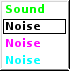
\includegraphics[scale=1.0]{1.6.0/voice_oscillator_sound_dropdown.png}
   \caption{Voice Oscillator Choices}
   \label{fig:voice_oscillator_choices}
\end{figure}

   \itempar{Waveform graph}{voice oscillator!waveform}
   Waveform Graph.
   Shows a period of the currently configured oscillator.

\begin{figure}[H]
   \centering
   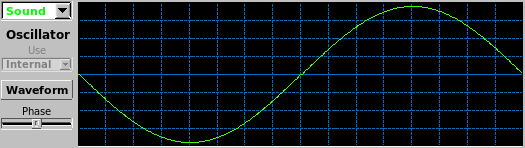
\includegraphics[scale=0.75]{1.5.7/sound_banner.png}
   \caption{Oscillator in ADDSynth Voice}
   \label{fig:voice_oscillator_oscillator}
\end{figure}

   If white \textbf{Noise} is selected, then the waveform graph simply announces
   "White Noise".  Also, the \textbf{Unison, Frequency, Modulator} controls are
   all disabled.

\begin{figure}[H]
   \centering
   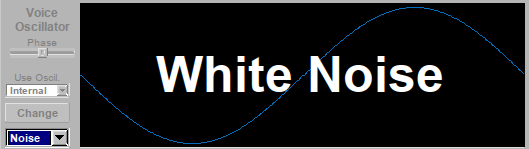
\includegraphics[scale=0.75]{1.5.7/white_noise_banner.png}
   \caption{White Noise in ADDSynth Voice}
   \label{fig:voice_oscillator_white_noise}
\end{figure}

   If the pink \textbf{Noise} entry is selected,
   then the waveform graph simply announces "Pink Noise".
   Also, the \textbf{Unison, Frequency, Modulator} controls are
   all disabled.

\begin{figure}[H]
   \centering
   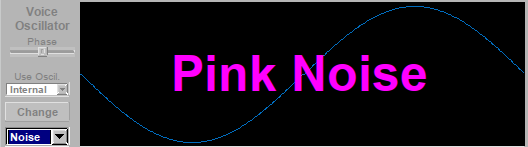
\includegraphics[scale=0.75]{1.5.7/pink_noise_banner.png}
   \caption{Pink Noise in ADDSynth Voice}
   \label{fig:voice_oscillator_pink_noise}
\end{figure}

\index{new!spot noise}
   If the cyan (spot) \textbf{Noise} entry is selected,
   then the waveform graph simply announces
   "Spot Noise".  Also, the \textbf{Unison, Frequency, Modulator} controls are
   all disabled.
   Spot noise is based on white noise but has a very broken sound. Combined with
   envelope shaping this is useful for adding 'grit' or sizzle, particularly for
   percussion.

\begin{figure}[H]
   \centering
   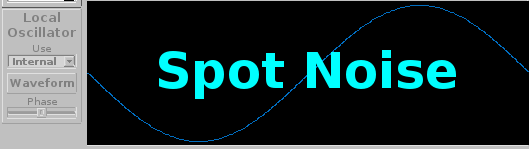
\includegraphics[scale=0.75]{1.6.0/spot_noise_banner.png}
   \caption{Spot Noise in ADDSynth Voice}
   \label{fig:voice_oscillator_spot_noise}
\end{figure}

   \itempar{Use (oscillator)}{voice oscillator!use}
   Use Oscillator.
   If the \textbf{Current Voice} is set to a value greater than 1, meaning
   that one is editing additional voices, then this dropdown item also
   includes the values of all oscillators less then this one, marked as
   "Voice n", where "n" is the voice number.
   For example, if one is currently editing current voice 3,
   then the dropdown list includes \textbf{Internal}, \textbf{Voice 1}, and
   \textbf{Voice 2}.

  Unlike Source, using an oscillator from a different voice
  only imports the waveform, not any other parameters.

   Values: \texttt{Internal*, Other oscillators ("Voice n")}

   \itempar{Waveform}{voice oscillator!Waveform}
   ADDSynth Voice Oscillator Waveform.
   This button brings up the ADDsynth Oscillator Editor dialog.
   This dialog is described elsewhere; it used to be called
   \textbf{Change}.

   \itempar{Phase}{voice oscillator!phase}
   Voice Oscillator Phase.

   Values: \texttt{-90, 0*, 88.6 (degrees)}

\subsubsection{ADDsynth / Voice Parameters / MODULATOR}
\label{subsubsec:addsynth_voice_parameters_modulator}

   \begin{enumber}
      \item \textbf{Type:}
      \item \textbf{Modulator Source}
      \item \textbf{Mod AMPLITUDE}
      \item \textbf{Mod FREQUENCY}
      \item \textbf{Local Oscillator}
   \end{enumber}

   \setcounter{ItemCounter}{0}      % Reset the ItemCounter for this list.

   \itempar{Type:}{modulator!type}
   ADDsynth Modulator Type.

\begin{figure}[H]
   \centering
   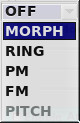
\includegraphics[scale=0.75]{bottom-panel/instrument-edit/ADD/modulator-type.jpg}
   \caption{Voice Modulator Type}
   \label{fig:voice_modulator_type}
\end{figure}

   \begin{enumber}
      \item \textbf{OFF}.
         This setting turns off the modulator.
      \item \textbf{MORPH}
         \index{MORPH}
         \index{morph modulator}
         \index{modulator!morph}
         The morph modulator works by combining the output of the voice oscillator
         and the modulator opscillator into one sonud, with the amplitude envelope
         translating between one waveform and the other. It is important that the
         amplitude envelope is enabled, otherwise no change will take place.

      \item \textbf{RING}
         \index{RING}
         \index{ring modulator}
         \index{modulator!ring}
         The ring modulator is useful for making bell-like sounds and some
         weird effects.  The ring modulator works by multiplying two
         waveforms together, producing a signal that possesses the sum and
         difference of the frequencies present in the waveforms.  The
         ins-and-outs of the ring modulator are explained in detail in
         \paragraphref{paragraph:tips_using_the_ring_modulator}.
      \item \textbf{PM}
         \index{PM}
         \index{phase modulator}
         \index{modulator!phase}
         The PM (phase modulation) modulator works by using a modulator
         envelope to change the phase of the voice oscillator. It produces a
         similar effect to frequency modulation.
         Generally, set \textbf{F.Damp} to zero, so that the modulation amount
         doesn't depend on the note number.
      \item \textbf{FM}
         \index{FM}
         \index{frequency modulator}
         \index{modulator!frequency}
         The (frequency modulation) morph modulator works by modulating the
         frequency.  Examples can be heard in the "Ethereal" and "Steel Wire"
         instruments.
      \item \textbf{PWM}
         \index{PWM}
         \index{PWM modulator}
         \index{modulator!PWM}
         The pulse width modulator works by pulse-width modulation.
   \end{enumber}

   Values: \texttt{OFF, MORPH, RING, PM, FM, PWM}

  \itempar{Modulator Source}.
  AddSynth Modulator Source.
  \index{modulator!source}
  Use another voice as a modulator instead of the modulator of the internal
  voice. One can make a "modulation stack". All parameters from the imported
  voice remain in effect, except for volume, panning, base frequency and pitch
  bend scaling factor. The voice is also converted to mono. Parameters in the
  current voice will then tweak the modulator further.
  One can only select Local (i.e. Internal), or one from a lower numbered voice.

   This feature allows one of the voices (of the up to 8 allowed in a single
   ADDsynth instrument) to be used as a modulator or external oscillator for
   another voice in the instrument.
   Note that the voice must be one with a number \textsl{below} the current
   voice.
   It's important to understand that oscillators always exist even if not
   used.
   \index{oscillator!local}
   This option specifies to use the oscillator of another voice or
   the \textsl{local} oscillator.

   Values: \texttt{Local*, "Mod n"}

   The parameters must be lower than the voice index; one cannot use the
   oscillator from a voice with a bigger index (e.g. one can't use the
   oscillator of voice 8 for voice 4). This is very useful because, if
   one uses many voices with the same oscillator settings, one can use only
   one oscillator and select other voices to use this, and if one changes a
   parameter of this oscillator, all voices using this oscillator will be
   affected.

   If one sets up voice 2 as a square wave, and voice 1 as a triangle wave,
   then sets voice 3 to voice 2, voice 3 will get a square wave.

   If one then sets voice 2 to voice 1, voice 2 will get a triangle wave but
   voice 3 will still get a square wave.

   Voice 3 can use the oscillator from voice 1,
   \textsl{even if voice 1 is switched off}.

   Modulator 3 can use the oscillator from modulator 1, even if modulator 1 is
   switched off, but modulator 3 can't use voice 1 if voice 1 is
   switched off.

   However, if voice 2 is using the oscillator from voice 1, and modulator 3 is
   using voice 2, it will still get voice 2 oscillator.

   When a voice or modulator is pointed to another voice/modulator, the
   oscillator window will show the waveform of the actual source, and all the
   controls will change this, not the internal oscillator.

   \textbf{Local}.
   Uses the local (internal) oscillator as the modulator of another voice.

   Values: \texttt{Local*, Other voice numbers}

   \itempar{Mod AMPLITUDE}{modulator!amplitude}
   Modulator Amplitude.

   \begin{enumber}
      \item \textbf{Vol}
         Volume.
         Values: \texttt{0 to 127, 90*}
      \item \textbf{V.Sns}
         Velocity Sensing Function; set to rightmost/max to disable.
         Values: \texttt{0 to 127, 64*}
      \item \textbf{F.Damp}
         Modulator Damp at higher frequency.
         How the modulator intensity is lowered according to lower/higher
         note frequencies.
         Values: \texttt{0 to 127, 90*}
      \item \textbf{Amplitude Env, Stock + Enable}
         See \sectionref{subsubsec:amplitude_envelope_subpanel}.
   \end{enumber}

   \itempar{Mod FREQUENCY}{modulator!frequency}
   Modulator Frequency.

% TODO FOR 1.6.0:  Uncomment the commented text.

   \begin{enumber}
     \item \textbf{Follow voice}
        Applies all detuning in the main voice oscillator to the modulator as
        well. If turned off, the modulator will be completely unaffected by all
        detuning in the main voice oscillator, including detuned unison voices.
     \item \textbf{440Hz}
        Use 440Hz as base frequency for the modulator.
      \item \textbf{Detune slider}
         Fine Detune (cents).
         Values: \texttt{-35.00 to 35.00, 0*}
      \item \textbf{Detune Type}
         Fine Detune (cents).
         Values: \texttt{L35cents, L10cents, E100cents, E1200cents}
         See \figureref{fig:addsynth_freq_detune_type}.
      \item \textbf{Octave}
         Octave.
         Values: \texttt{-8 to 7, 0*}
      \item \textbf{Coarse Det.}
         Coarse Detune.
         Values: \texttt{-64 to 63, 0*}
      \item \textbf{Filter Env, Stock + Enable}
         See \sectionref{subsubsec:envelope_settings_for_filter}.
   \end{enumber}

   \itempar{Local Oscillator}{modulator!oscillator}
   Local Oscillator.
   Provides the modulator for the oscillator.
   This value must indicate a modulator from a voice with a number less than
   the current voice. Entries are greyed out for Voice 1, as there is no
   lower-numbered voice available for modulation.

   Values: \texttt{Internal*, "Mod n"}

   \begin{enumber}
      \item \textbf{Waveform}
         ADDsynth Oscillator Editor.
      \item \textbf{Use}
         Oscillator to Use.
         See the paragraph below.
         Values: \texttt{Internal*, Other oscillators?}
      \item \textbf{Phase}
         Oscillator Phase.

         Values: \texttt{-90, 0*, 88.6 (degrees)}
      \item \textbf{Waveform graph}
         Waveform graph.
   \end{enumber}

   One has the choice between \textbf{Internal}, which in this case means a
   completely independent modulator oscillator per voice (extra waveform button),
   or \textbf{Mod. (n)}, which refers to the modulation oscillators one has
   already defined for the voices with a lower index.
   The voice of lower index doesn't need to be enabled in order to be used as a
   modulator. This means one can make one modulation oscillator for voice 1, and
   reuse it in voices 2 and 3.  This is the same system used for the normal (voice)
   oscillators.

\paragraph{Tip: Using the Ring Modulator}
\label{paragraph:tips_using_the_ring_modulator}
\index{tips!ring modulator}
\index{tips!internal modulator}

   This section is derived from one of the short text files in the
   \textsl{Yoshimi} source-code bundle (\cite{yoshimi} or \cite{yoshimi2}).
   It notes that "Some people have
   been confused about how to use an 'external' Mod Oscillator", and
   provides usage notes that we will elaborate on here.  Here is the way to
   use the ring modulator:

   \begin{enumber}
      \item Open the ADDsynth editing window.  Then open
         \textbf{Show Voice Parameters}.
      \item For \textbf{Type}, select the \textbf{RING} value.  This
         selection will activate the \textbf{Mod Oscillator}.
      \item In the \textbf{Local Oscillator}, click on \textbf{Waveform} to open
         the \textbf{ADDsynth Oscillator Editor}.
      \item Set the wave-shape to \textbf{Triangle}.
      \item Switch to voice number 2 and enable it.
      \item Again, for \textbf{Type}, select the \textbf{RING} value.
         However, feel free to select one of the other modulators, if one
         wishes.
      \item One can now use \textbf{Internal} for voice 2, or select
         \textbf{Voice} 1, to use the first voice as in internal modulator.
      \item Change the internal voice to, for example, \textbf{Square}.
      \item Do the same setup for voice 3.
         One will find that one can use its \textbf{Internal} or
         either of the two previous ones.
   \end{enumber}

   Now the joker in the pack is that one can disable both the previous
   voices but \textsl{still} use their Mod Oscillators.

   In a newsgroup (\cite{ringmodulator}, the following note is found.

   \begin{quotation}
      Say I want the A tone ring-modulated by 880Hz. A is 440 Hz, the ring
      modulation setting lets me choose the modulation frequency relative
      to the frequency of the tone. So I choose octave 1 and let the
      detune at zero. If I move the detune, it'll shift the modulation
      frequency a bit, which will make a disharmonic effect.

      Wet/dry setting is controlled by volume in "modulation amplitude".
      The modulation frequency can further be multiplied or several
      modulations can be simulated by changing the oscillator waveform.

      One huge letdown is that it is only available for Adsynth. PadSynth
      does not seem to have ring modulation option, so the coolest sounds
      stay out of question for massive lead tones. :-(
   \end{quotation}

   We have provided a more useful "tutorial" on using the ring modulator in the
   \textsl{Yoshimi Cookbook} \cite{cookbook} document.

   Finally, at the bottom of the ADDsynth Voice Part dialog, (under the Modulator
   section, we find the last few controls.

   \setcounter{ItemCounter}{0}      % Reset the ItemCounter for this list.

   \itempar{C}{voice oscillator!copy}
   Copy D note parameters ("DnoteParameters").

   \itempar{P}{voice oscillator!paste}
   Paste D note parameters ("DnoteParameters").

   \itempar{Close Window}{voice oscillator!close}
   Close.


\subsection{ADDsynth / Voice List}
\label{subsec:addsynth_voice_list}

   The ADDsynth Voices List shows a summary of voices 1 to 8, and allows
   some overall control of them, almost like a simple mixer.
   It is brought on-screen via the \textbf{Show Voice List} button
   of the ADDsynth global part editor.
   It is fully in sync with the voice windows.

\begin{figure}[H]
   \centering
   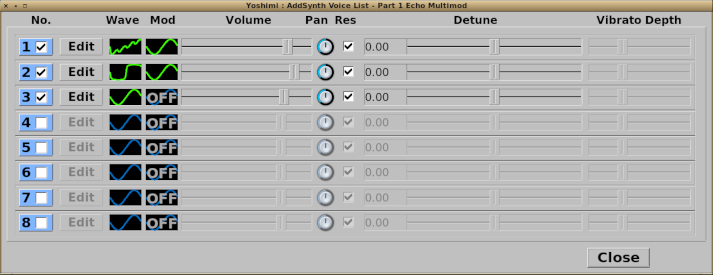
\includegraphics[scale=0.75]{2.0/AddSynthVoiceList.png}
   \caption{ADDsynth Voices List}
   \label{fig:addsynth_voices_list}
\end{figure}

   \begin{enumber}
      \item \textbf{No. (1 to 8)}
      \item \textbf{Edit}
      \item \textbf{Wave}
      \item \textbf{Mod}
      \item \textbf{Vol}
      \item \textbf{Pan}
      \item \textbf{Res}
      \item \textbf{Detune}
      \item \textbf{Vibrato Depth}
      \item \textbf{Hide Voice List}
   \end{enumber}

   \setcounter{ItemCounter}{0}      % Reset the ItemCounter for this list.

   \itempar{No. (1 to 8)}{voice list!number}
   Voice List Number.
   This check-box enables or disables a given voice in the current part.

   Values: \texttt{Off, On}

   \itempar{Edit}{voice list!edit}
   ADDSynth Voice List Edit Button.
   This button brings up the appropriate ADDSynth Voice dialog so that the
   waveform can be easily brought up for modification.

   \itempar{Wave Icon}{voice list!waveform icon}
   Waveform Icon.
   The waveform icon shows a rough rendering of the actual shape of the voice
   waveform, or the letter \textbf{N} is the voice is constructed from white
   noise, or the letters \textbf{O} or \textbf{V} followed by a number if the
   voice is using an external oscillator or voice input, respectively.
   Note that this picture isn't updated if the voice is edited, until the voice
   list is closed and reopened.

% TODO FOR 1.6.0:  Uncomment the commented text.

  \itempar{Modulation Icon}{voice list!modulation icon}
  Modulation Icon.
  The modulation icon shows a rough rendering of the actual shape of the voice
  modulation, or the letters \textbf{M} or \textbf{V} followed by a number if
  the voice is using an external modulator oscillator or voice input,
  respectively.
  Note that this picture isn't updated if the voice is edited, until the voice
  list is closed and reopened.

   \itempar{Vol}{voice list!volume}
   Voice Volume.
   This slider controls the relative volume of a given voice in the current
   part.

   Values: \texttt{0 to 127, 100*}

   \itempar{Pan}{voice list!panning}
   Voice Panning (0/leftmost is Random).
   This slider controls the panning of a given voice in the current part.

   Values: \texttt{0 to 127, 64*}

   \itempar{Res}{voice list!resonance}
   Resonance On/Off.
   Enable/disable the resonance effect of a voice.
   Note that the resonance is configured in by the Resonance dialog brought
   up by the \textbf{Resonance} button at the bottom of the ADDsynth main
   dialog.  The resonance dialog has its own Enable button, as well.
   This is provided so individual voices can bypass the resonance filter.

   Values: \texttt{Off, On*}

   \itempar{Detune Value}{voice list!detune value}
   This read-only text-box shows the current value of detune as selected by
   its slider.

   \itempar{Detune}{voice list!detune}
   Fine Detune (cents).

   Values: \texttt{-35 to 35, 0*}

   \itempar{Vibrato Depth}{voice list!vibrato depth}
   Frequency LFO Amount/Depth.
   This setting can be very useful because, with the detune settings, one can
   create very good sounding instruments.

   Values: \texttt{0 to 127, 40*}

   \itempar{Hide Voice List}{voice list!hide}
   Hide Voice List.  A Close button, really, and that is what it is in the
   latest version of \textsl{Yoshimi}.

\subsection{ADDsynth / Oscillator}
\label{subsec:addsynth_oscillator}

   Pressing the \textbf{Waveform} button in the ADDsynth
   voice-editor dialog brings up a very complex dialog for modifying the
   harmonics of the voice.

\begin{figure}[H]
   \centering
   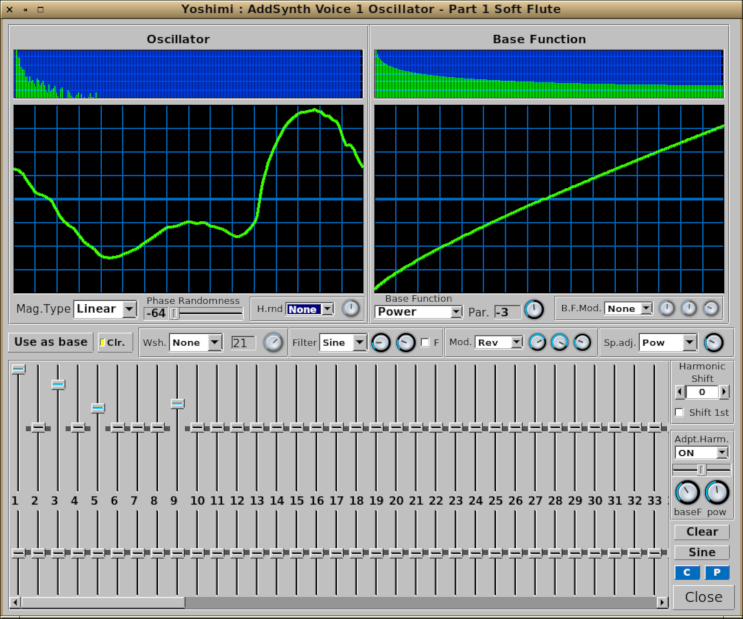
\includegraphics[scale=0.75]{2.0/Oscillator.png}
   \caption{ADDsynth Oscillator Editor}
   \label{fig:addsynth_oscillator_editor}
\end{figure}

   This item is nearly identical to the PADsynth harmonic editor depicted in
   \figureref{fig:padsynth_harmonic_content_editor},
   except for the items noted below.
   Obviously, it is a topic unto itself!

   \begin{enumber}
      \item \textbf{Oscillator Spectrum Graph}
      \item \textbf{Oscillator Waveform Graph}
      \item \textbf{Mag.Type}
      \item \textbf{Phase Randomness} (ADDsynth Oscillator Editor only)
      \item \textbf{H.rnd} (ADDsynth Oscillator Editor only)
      \item \textbf{H.rnd knob} (ADDsynth Oscillator Editor only)
   \end{enumber}

   \setcounter{ItemCounter}{0}      % Reset the ItemCounter for this list.

   \itempar{Oscillator Spectrum Graph}{addsynth!oscillator graph}
   Oscillator Spectrum Graph.
   This graph shows the spectrum of the oscillator as a series of vertical
   lines, a kind of frequency histogram.

   \itempar{Oscillator Waveform Graph}{addsynth!waveform graph}
   Oscillator Waveform Graph.
   This graph shows the temporal waveform  of the oscillator.

   \itempar{Mag.Type}{addsynth!mag type}
   Oscillator Magnitude Type.
   Sets how the magnitudes from the user interface behave.  See the values
   below.

   \itempar{Phase Randomness}{addsynth!rnd}
   Phase Randomness. Sets the randomness of the oscillator phase which is
   settable from -64 (-90 deg) to 63 (+90 deg).

   \itempar{H.rnd}{addsynth!H.rnd}
   Harmonic Amplitude Randomness.
   Enables the feature and sets the 'law' for the way randomness is applied.

\begin{figure}[H]
   \centering
   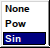
\includegraphics[scale=1.0]{bottom-panel/instrument-edit/ADD/ADDsynth-hrnd.png}
   \caption{ADDsynth Oscillator Harmonic Randomness Selections}
   \label{fig:addsynth_hrnd}
\end{figure}

   Values: \texttt{None, Pow, and Sin}

   \itempar{H.rnd knob}{addsynth!H.rnd knob}
   Harmonic Amplitude Randomness Knob.
   Adjusts the amount of randomness applied to the amplitudes of individual harmonics.

   Values: \texttt{0 to 127, 64*}

\subsection{ADDsynth / Voice Warning}
\label{subsec:addsynth_voice-warning}
   As of V 1.5.11 there is a warning about editing waveforms.

   When editing an AddSynth voice that is taking it's waveform from another one
   the 'Waveform' text turns blue as a warning. However when actually entering
   the waveform window iteself, until now there was no indication that one was
   likely to change a shared oscillator. This is put right since V 1.5.11 and
   it also applies to modulator waveforms.

\begin{figure}[H]
   \centering
   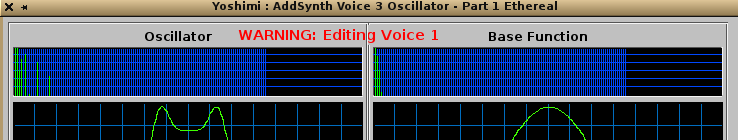
\includegraphics[scale=0.75]{1.5.11/oscillator_warning.png}
   \caption{Warning in ADDSynth Oscillator}
   \label{fig:voice_oscillator_warning}
\end{figure}

   As can be seen, not only does one see the warning, but also exactly which
   voice (or modulator) is being edited.

\subsection{ADDsynth / Resonance}
\label{subsec:addsynth_resonance}

   This dialog, shared in common with the PADsynth editor, is a stock
   user-interface element described in
   \sectionref{subsec:stock_resonance_settings}.

%-------------------------------------------------------------------------------
% vim: ts=3 sw=3 et ft=tex
%-------------------------------------------------------------------------------
